\documentclass[a4paper,11pt]{article} \usepackage[T1]{fontenc} \usepackage[utf8]{inputenc} \usepackage[francais]{babel}
\usepackage[top=2cm,left=2.5cm,right=2.5cm,bottom=2cm]{geometry} % Géométrie de la page, modifier selon le besoin
\usepackage{xcolor}
\usepackage{listingsutf8}
\usepackage{textcomp}
\usepackage{float}
%\usepackage{minted}
%décommente pas sauf si tu sais résoudre l'erreur de compile qui en résulte
\lstset{
    language=C++,
    keywordstyle=\bfseries\ttfamily\color[rgb]{0,0,1},
    identifierstyle=\ttfamily,
    commentstyle=\color[rgb]{0.133,0.545,0.133},
    stringstyle=\ttfamily\color[rgb]{0.627,0.126,0.941},
    showstringspaces=false,
    basicstyle=\small,
   % numberstyle=\footnotesize,
    %numbers=left,
    %stepnumber=1,
    %numbersep=10pt,
    %j'aime pas afficher les numéros de ligne vu qu'on met que des extraits de code
    tabsize=2,
    breaklines=true,
    prebreak = \raisebox{0ex}[0ex][0ex]{\ensuremath{\hookleftarrow}},
    breakatwhitespace=false,
    aboveskip={\baselineskip},
  columns=fixed,
  upquote=true,
  extendedchars=true,
  inputencoding=utf8/latin1
}


\lstset{language=C++}
\usepackage{lmodern, wrapfig, textcomp, tikz, graphicx}





\begin{document}
\begin{titlepage}
%
\includegraphics[scale=0.45]{Images/logo_phelma.pdf}\hfill
\begin{center}
    \vspace*{1cm}
    \textsc{\Large Bureau d'Études d'Informatique}\\
    [4.5cm] \rule{\linewidth}{0.5mm}\\[0.4cm]
    {\huge\bfseries Fractales et FLTK\\
    [0.4cm]}\rule{\linewidth}{0.5mm}\\[1.0cm]
    \textsc{pmpB}
    \begin{flushright} \large
        % \emph{Entrepreneurs :} \\
        Julia \textsc{Dupuis}\\
        Nils \textsc{Exibard}\\
        Félix \textsc{Piédallu}\\
    \end{flushright}
    
    
  \begin{center}
    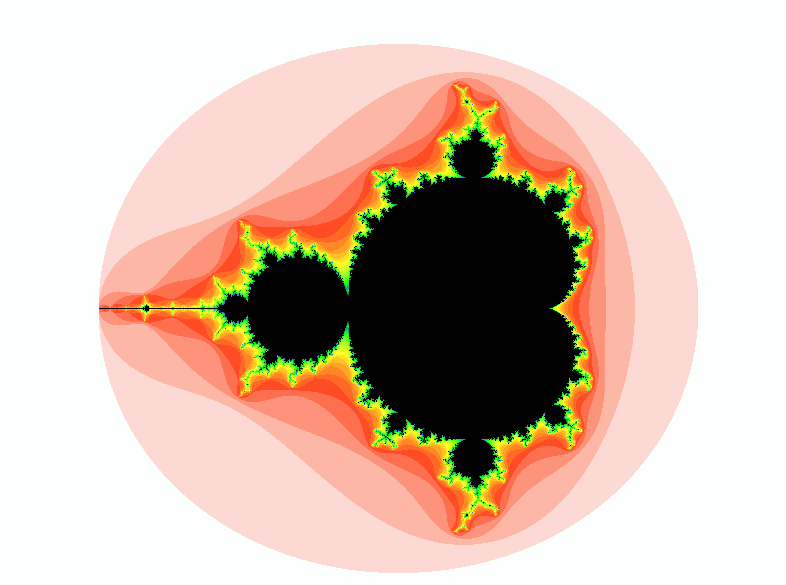
\includegraphics[width=0.7\textwidth]{Images/Titlepage.png}
  \end{center}

    \vfill

    \large{\today}
\end{center}
\end{titlepage}
     % Fichier de page de titre
\tableofcontents          % Table des matières avec liens, générée automatiquement.
\vspace{3cm}
%\input{0.Intro.tex}
%tu vireras ce comment quand t'auras rajouté le tex correspondant, fait que ça compile
\newpage

\section{Présentation du programme}
Le sujet  sur lequel nous avons choisi de travailler est le projet « Fractales », grand classique de la programmation, utilisant le plan complexe.
\begin{figure}[H] \begin{center} 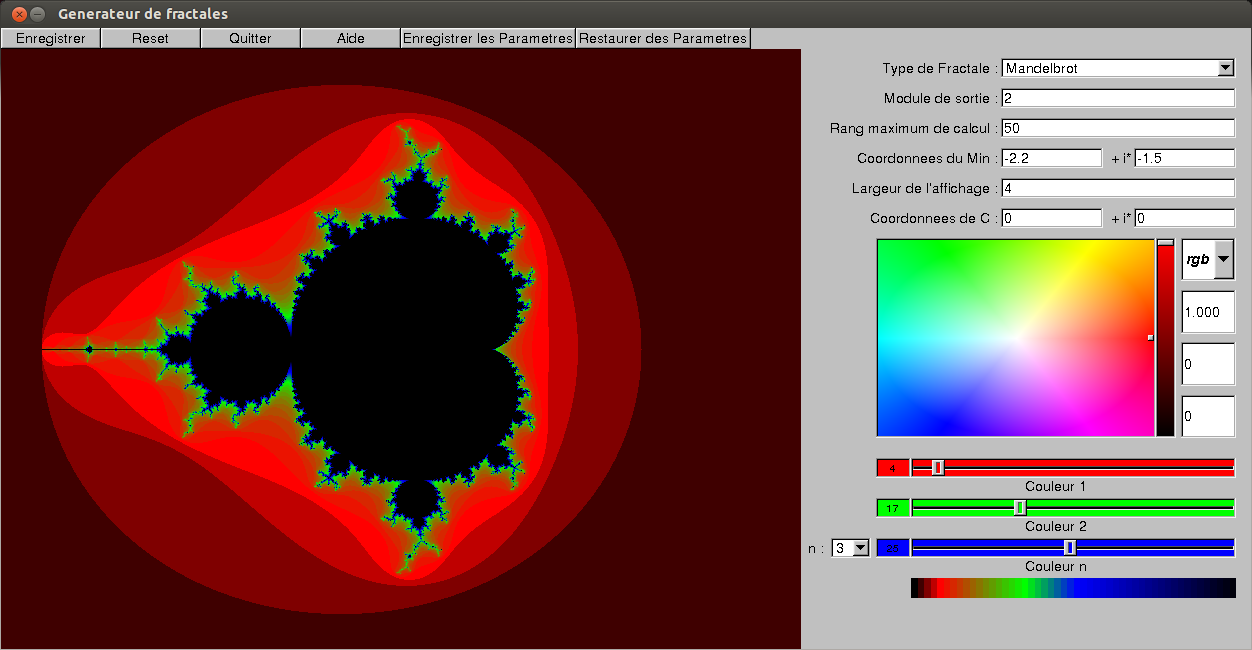
\includegraphics[width=\textwidth]{Images/InterfaceTotale.png}
    \caption{}
\end{center} \end{figure}

Les fonctionnalités que nous avons choisi d'intégrer sont les suivantes :
\begin{itemize}
  \item Choix par l’utilisateur des différents paramètres de la fractale (type, module de sortie, rang maximal, coordonnées du point inférieur gauche, largeur de l’affichage, coordonnées de la constante).
        \begin{figure}[H] \begin{center} 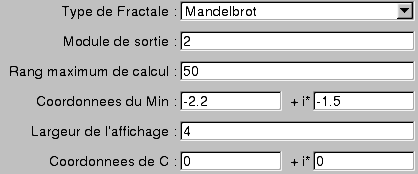
\includegraphics[width=0.5\textwidth]{Images/Parametres.png}
            \caption{}
        \end{center} \end{figure}


  \item Choix des couleurs (jusqu'a 10 couleurs choisies par l’utilisateur avec écart modifiable).
        \begin{figure}[H] \begin{center} 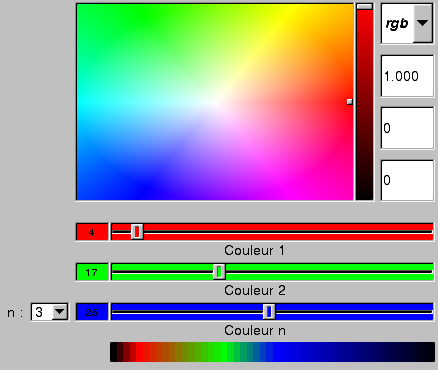
\includegraphics[width=0.5\textwidth]{Images/ChoixCouleurs.png}
            \caption{}
        \end{center} \end{figure}
  \item Enregistrement de l’image ainsi que des paramètres dans un fichier choisi par l’utilisateur avec une qualité choisie.
  \item Restauration de paramètres précédemment enregistrés.
  \item Remise à zéro des paramètres (bouton reset).
  \item Fonction « Quitter ».
  \item Un bouton aide expliquant les fonctionnalités des différents boutons de la souris.
        \begin{figure}[H] \begin{center} 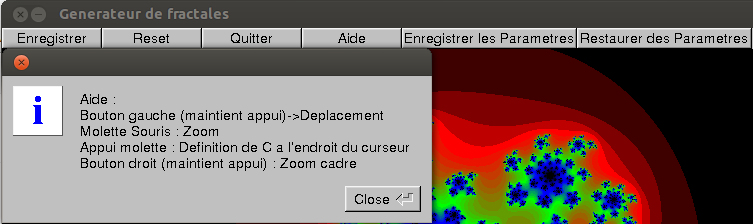
\includegraphics[width=0.8\textwidth]{Images/Aide.png}
            \caption{}
        \end{center} \end{figure}
  \item 2 types de zoom : avec cadre(clic droit) ou grâce à la molette .
        \begin{figure}[H] \begin{center} 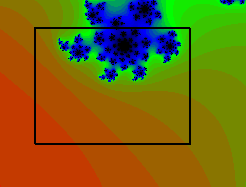
\includegraphics[width=0.5\textwidth]{Images/Cadre.png}
            \caption{}
        \end{center} \end{figure}
  \item Déplacement de l’image (clic gauche maintenu).
\end{itemize}



\section{Sources}

\subsection{Affichage}%à remplir

\subsection{Structures de données}
\begin{lstlisting}
struct Pixel {
    complex<double> z;      //Coordonnées du pixel dans le plan complexe
    int n;                  //Rang de divergence du pixel
};
\end{lstlisting}
Cette structure permettra de tracer la fractale à partir du rang de divergence et de la coordonnée de chaque pixel.
\begin{lstlisting}
struct Donnees {
    enum fractype Fractale; // Type de fractales choisie (Type énuméré)
    int     rangMax;        // Rang maximal de convergence
    double  moduleMax;      // Module de convergence (determination de la convergence on non de la fonction)
    complex<double> C;      // Constante de calcul
    complex<double> ig;     // Coordonnees du point inferieur gauche
    double pasxy;           // Pas de la matrice (incrementation, en fait, et egale dans les 2 dimensions, car pixels carres)
    struct Pixel Tab[L_ZONE][H_ZONE]; // Matrice des pixels de l'image.
int hauteur;             //Hauteur de l'image
    unsigned char buffer[3*L_ZONE*H_ZONE];//contient l'image sous forme RGB
    unsigned char bufferDeg[3*325];//contient l'apperçu du dégradé sous forme RGB
    int nbSlider;           //Nombre de slider actifs
    unsigned long int slider[MAX_SLIDER+2][2];//contient le rang et la couleur de chaque slider
};

\end{lstlisting}
Cette structure est la plus importante du programme.

\begin{lstlisting}
struct Tests {
    bool dessin;//faut-il refaire le dessin?
    bool calcul;//faut il refaire le calcul
    bool calccouleurs;//faut il refaire le calcul des couleurs ?
    int slider; //contient le slider actif
};
\end{lstlisting}
Cette structure contient les variables nécessaires à la vérification des conditions, cela permet entre autre d’éviter les calculs inutiles.

\begin{lstlisting}
enum fractype {
    MANDELBROT,
    JULIA,
    COSC,
    SINZO,
    PERSONNA//Originellement prévue pour une fractale personnalisée, non utilisée faute de temps
};
\end{lstlisting}
Le type énuméré permet d'utiliser plus facilement les différents types de fractales.


\subsection{Fonctions }
\begin{lstlisting}
void InitialiserDonnees() ;
\end{lstlisting}
Initialise les données du programmes
\begin{lstlisting}
void realFromTab(double *bi, double *bj);
\end{lstlisting}
Effectue la correspondance entre les coordonnées complexe et les pixels
\begin{lstlisting}
pointeurFct retourne_fonction();    // Pointe vers les fonctions suivantes en fonction de la fractale choisie
\end{lstlisting}
%Félix t'expliqueras ça probab mieux que moi
\begin{lstlisting}
int mandelbrot(complex<double> position);
int julia     (complex<double> position);
int sinzo     (complex<double> position);
int cosc      (complex<double> position);
int personna  (complex<double> position);
\end{lstlisting}
Ce sont les algorithmes de calcul de convergence
\begin{lstlisting}
void convergenceLigne(int j, pointeurFct fonction);
\end{lstlisting}
Etudie la convergence ligne par ligne
\begin{lstlisting}
void degradeRGB(unsigned long int A, unsigned long int  B,int N, int tab[][3]);
\end{lstlisting}
Effectue le calcul d'un dégradé de taille N entre une couleur A et une couleur B, et stocke les trois composantes RGB dans tab
\begin{lstlisting}
void couleursRGB(unsigned long tabSlider[][2],int tab[][3]) ;
\end{lstlisting}
Remplis tab d'une suite de dégradé grace à degradeRGB à partir des informations contenues dans tabSlider
\begin{lstlisting}
void calcBuffer(int tabdeg[][3]);
\end{lstlisting}
calcule et stocke dans gDonnees.bufferDeg a partir d'un tableau de couleurs RGB
\begin{lstlisting}
int enregistrerPPM(int Largeur, char Fichier[32]);
\end{lstlisting}
Enregistre une image en ppm de Largeur pixel de large et de ratio constant dans Fichier.
\begin{lstlisting}
void enregistrerParams(const char* fichier);
void restaurerParams(const char* fichier);
\end{lstlisting}
Permet d'enregistrer (et de lire, mais non finalisé) les paramètres permettants de redéssiner la fractale

\subsection{Dessin}
\begin{lstlisting}
void ZoneDessinInitialisation(Fl_Widget* widget, void* data);
\end{lstlisting}
%Initialise la zone de dessin puis appelle gestionAffichage_iter
\begin{lstlisting}
void afficheFractaleLigne();
\end{lstlisting}
Commande le calcul puis l'affichage d'une ligne
\begin{lstlisting}
void afficheLigneRGB(int j, int tableauCouleurs[][3]);
\end{lstlisting}
Affiche la ligne j avec pour couleurs un tableau RGB
\begin{lstlisting}
void gestionAffichage_iter(void* data);//iter car en remplacement de la fonction récursive d'origine.
\end{lstlisting}
Calcule SI nécéssaire la fractale puis l'affiche grace aux diverses autres fonctions.
\begin{lstlisting}
void tracerCadre (int x1, int y1 , int x2, int y2);
\end{lstlisting}
Trace le cadre du zoom cadre a partir de 2 points (conserve le ratio d'écran)
\begin{lstlisting}
void zoneDegrade(Fl_Widget* widget, void* data);
\end{lstlisting}
Gère l'affichage de la zone d’aperçu du dégradé

\subsection{Callback}%à remplir



\section{Critique}

%En vrac, à retravailler mais l'idée est la : 
\begin{itemize}
\item La fonction d'affichage est chaotique, elle appelle d'abord initialiser affichage qui appelle elle même gestionAffichage\_iter.% Si je me souviens bien ça évitait un bug fut un temps, Félix, je te laisse en parler.
\item La structure de données initiale pour les couleurs, qui limitaient le programme à 3 sliders. Il a fallu réécrire beaucoup de choses pour pouvoir augmenter le nombre de slider (maintenant on peut potentiellement mettre autant de point de couleurs que l'on veut)
\item Le tableau contenant le dégradé n'est pas alloué dynamiquement->soit on utilise un très grand tableau en variable globale, soit on le recalcule dès qu'on en a besoin (option choisie, cela entraîne quelques calculs supplémentaire mais de temps faible devant le calcul de la fractale)
\item Le programme ne fonctionne pas uniquement en RGB, mais on utilise un peu Fl\_Color, car nous nous sommes rendus compte après avoir tout implémenté avec Fl\_Color qu'il existait des accesseurs permettant d’accéder directement aux composantes RGB.\\
Certains algorithmes ont étés réécris en RGB, qui est bien plus pratique à se représenter, mais aussi pour écrire dans des buffer (nous avons abandonnés l'affichage point par point avec Fl\_point pour utiliser Fl\_draw\_image, bien plus rapide).
\item La gestion du multithreading, commencée mais abandonnée faute de temps (fonctionnait pour le calcul mais produisait des erreurs pour l'affichage).
\item La gestion des animations (couleurs variable) a été commencée, mais ayant a l'époque un problème d'affichage (passage par un écran noir a chaque nouveau dessin à cause de l'appel de la fonction "initialiser\_affichage", le résultats était peu convainquant. Après résolution du problème, nous n'avons pas eu le temps de la ré-implémenter.
\end{itemize}


\section{Déroulement du projet}
%Je sais pas trop quoi mettre la dedans, mais je vais essayer quand même :
Nous avions à l'origine effectué une répartition des taches (Julia pour l'interface et les Callbacks, Nils pour la gestion des couleurs, et Félix pour l'algorithmique des fractales et l'affichage). Cette répartition a été dans l'ensemble tenue,pour la base du programme, mais ensuite chaque nouvelle fonctionnalité a été codé intégralement par celui qui voulait l'implémenter, sans refaire de répartition des taches. 



\section{Conclusion}
%Hésitez pas à completer ou réecrire
Coder un programme entier s'est révélé très intéressant même si très coûteux en temps, surtout pour arriver à une interface assez intuitive (si l'on connaît un minimum le vocabulaire des fractales) et efficace.
Cela nous a permis de comprendre l'architecture d'un programme basé sur plusieurs fichiers et l'importance des structures de données. En effet, avec le recul, nos choix initiaux ne paraissent pas toujours optimaux, notamment si l'on veux modifier ou ajouter certaines fonctions (par exemple, il a fallu recoder beaucoup de chose pour passer à plus de trois point de couleurs, ce qui aurait pu être évité en choisissant une autre structure de donnée des le départ).
\end{document}